% Title: gl2ps_renderer figure
% Creator: GL2PS 1.4.0, (C) 1999-2017 C. Geuzaine
% For: Octave
% CreationDate: Thu Nov 28 00:22:14 2019
\setlength{\unitlength}{1pt}
\begin{picture}(0,0)
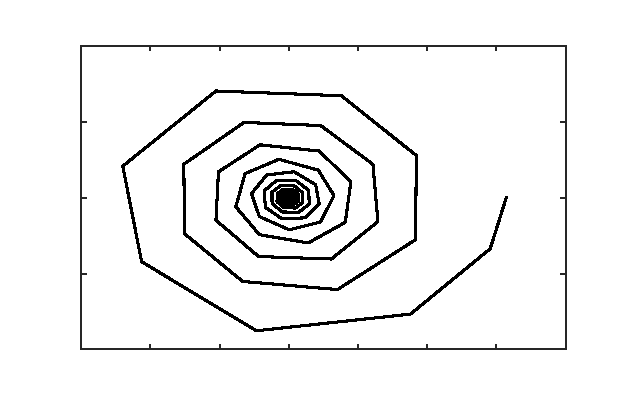
\includegraphics{../Report/img/faseF-inc}
\end{picture}%
\begin{picture}(300,200)(0,0)
\fontsize{10}{0}
\selectfont\put(39,25){\makebox(0,0)[t]{\textcolor[rgb]{0.15,0.15,0.15}{{-1.5}}}}
\fontsize{10}{0}
\selectfont\put(72.2143,25){\makebox(0,0)[t]{\textcolor[rgb]{0.15,0.15,0.15}{{-1}}}}
\fontsize{10}{0}
\selectfont\put(105.429,25){\makebox(0,0)[t]{\textcolor[rgb]{0.15,0.15,0.15}{{-0.5}}}}
\fontsize{10}{0}
\selectfont\put(138.643,25){\makebox(0,0)[t]{\textcolor[rgb]{0.15,0.15,0.15}{{0}}}}
\fontsize{10}{0}
\selectfont\put(171.857,25){\makebox(0,0)[t]{\textcolor[rgb]{0.15,0.15,0.15}{{0.5}}}}
\fontsize{10}{0}
\selectfont\put(205.071,25){\makebox(0,0)[t]{\textcolor[rgb]{0.15,0.15,0.15}{{1}}}}
\fontsize{10}{0}
\selectfont\put(238.286,25){\makebox(0,0)[t]{\textcolor[rgb]{0.15,0.15,0.15}{{1.5}}}}
\fontsize{10}{0}
\selectfont\put(271.5,25){\makebox(0,0)[t]{\textcolor[rgb]{0.15,0.15,0.15}{{2}}}}
\fontsize{10}{0}
\selectfont\put(34.0107,32.4756){\makebox(0,0)[r]{\textcolor[rgb]{0.15,0.15,0.15}{{-8}}}}
\fontsize{10}{0}
\selectfont\put(34.0107,53.2648){\makebox(0,0)[r]{\textcolor[rgb]{0.15,0.15,0.15}{{-6}}}}
\fontsize{10}{0}
\selectfont\put(34.0107,74.054){\makebox(0,0)[r]{\textcolor[rgb]{0.15,0.15,0.15}{{-4}}}}
\fontsize{10}{0}
\selectfont\put(34.0107,94.8432){\makebox(0,0)[r]{\textcolor[rgb]{0.15,0.15,0.15}{{-2}}}}
\fontsize{10}{0}
\selectfont\put(34.0107,115.632){\makebox(0,0)[r]{\textcolor[rgb]{0.15,0.15,0.15}{{0}}}}
\fontsize{10}{0}
\selectfont\put(34.0107,136.422){\makebox(0,0)[r]{\textcolor[rgb]{0.15,0.15,0.15}{{2}}}}
\fontsize{10}{0}
\selectfont\put(34.0107,157.211){\makebox(0,0)[r]{\textcolor[rgb]{0.15,0.15,0.15}{{4}}}}
\fontsize{10}{0}
\selectfont\put(34.0107,178){\makebox(0,0)[r]{\textcolor[rgb]{0.15,0.15,0.15}{{6}}}}
\fontsize{11}{0}
\selectfont\put(155.25,12){\makebox(0,0)[t]{\textcolor[rgb]{0.15,0.15,0.15}{{Posición ($\theta$)}}}}
\fontsize{11}{0}
\selectfont\put(20.0107,105.238){\rotatebox{90}{\makebox(0,0)[b]{\textcolor[rgb]{0.15,0.15,0.15}{{Velocidad ($\dot{\theta}$)}}}}}
\fontsize{11}{0}
\selectfont\put(155.25,188){\makebox(0,0)[b]{\textcolor[rgb]{0,0,0}{{Retrato fase $\theta / \dot{\theta}$}}}}
\end{picture}
